\chapter{Experimental Analysis}

This chapter presents the experimental setup, training behavior, evaluation metrics, and visual analysis of the house price prediction model.

The model was trained using a fully connected neural network architecture for 100 epochs with a batch size of 32. The Adam optimizer was used with an initial learning rate of 0.001, and the loss function selected was Mean Squared Error (MSE), appropriate for regression tasks. Training and validation losses were continuously monitored throughout the training phase to ensure model stability and prevent overfitting.

\begin{figure}[h]
\centering
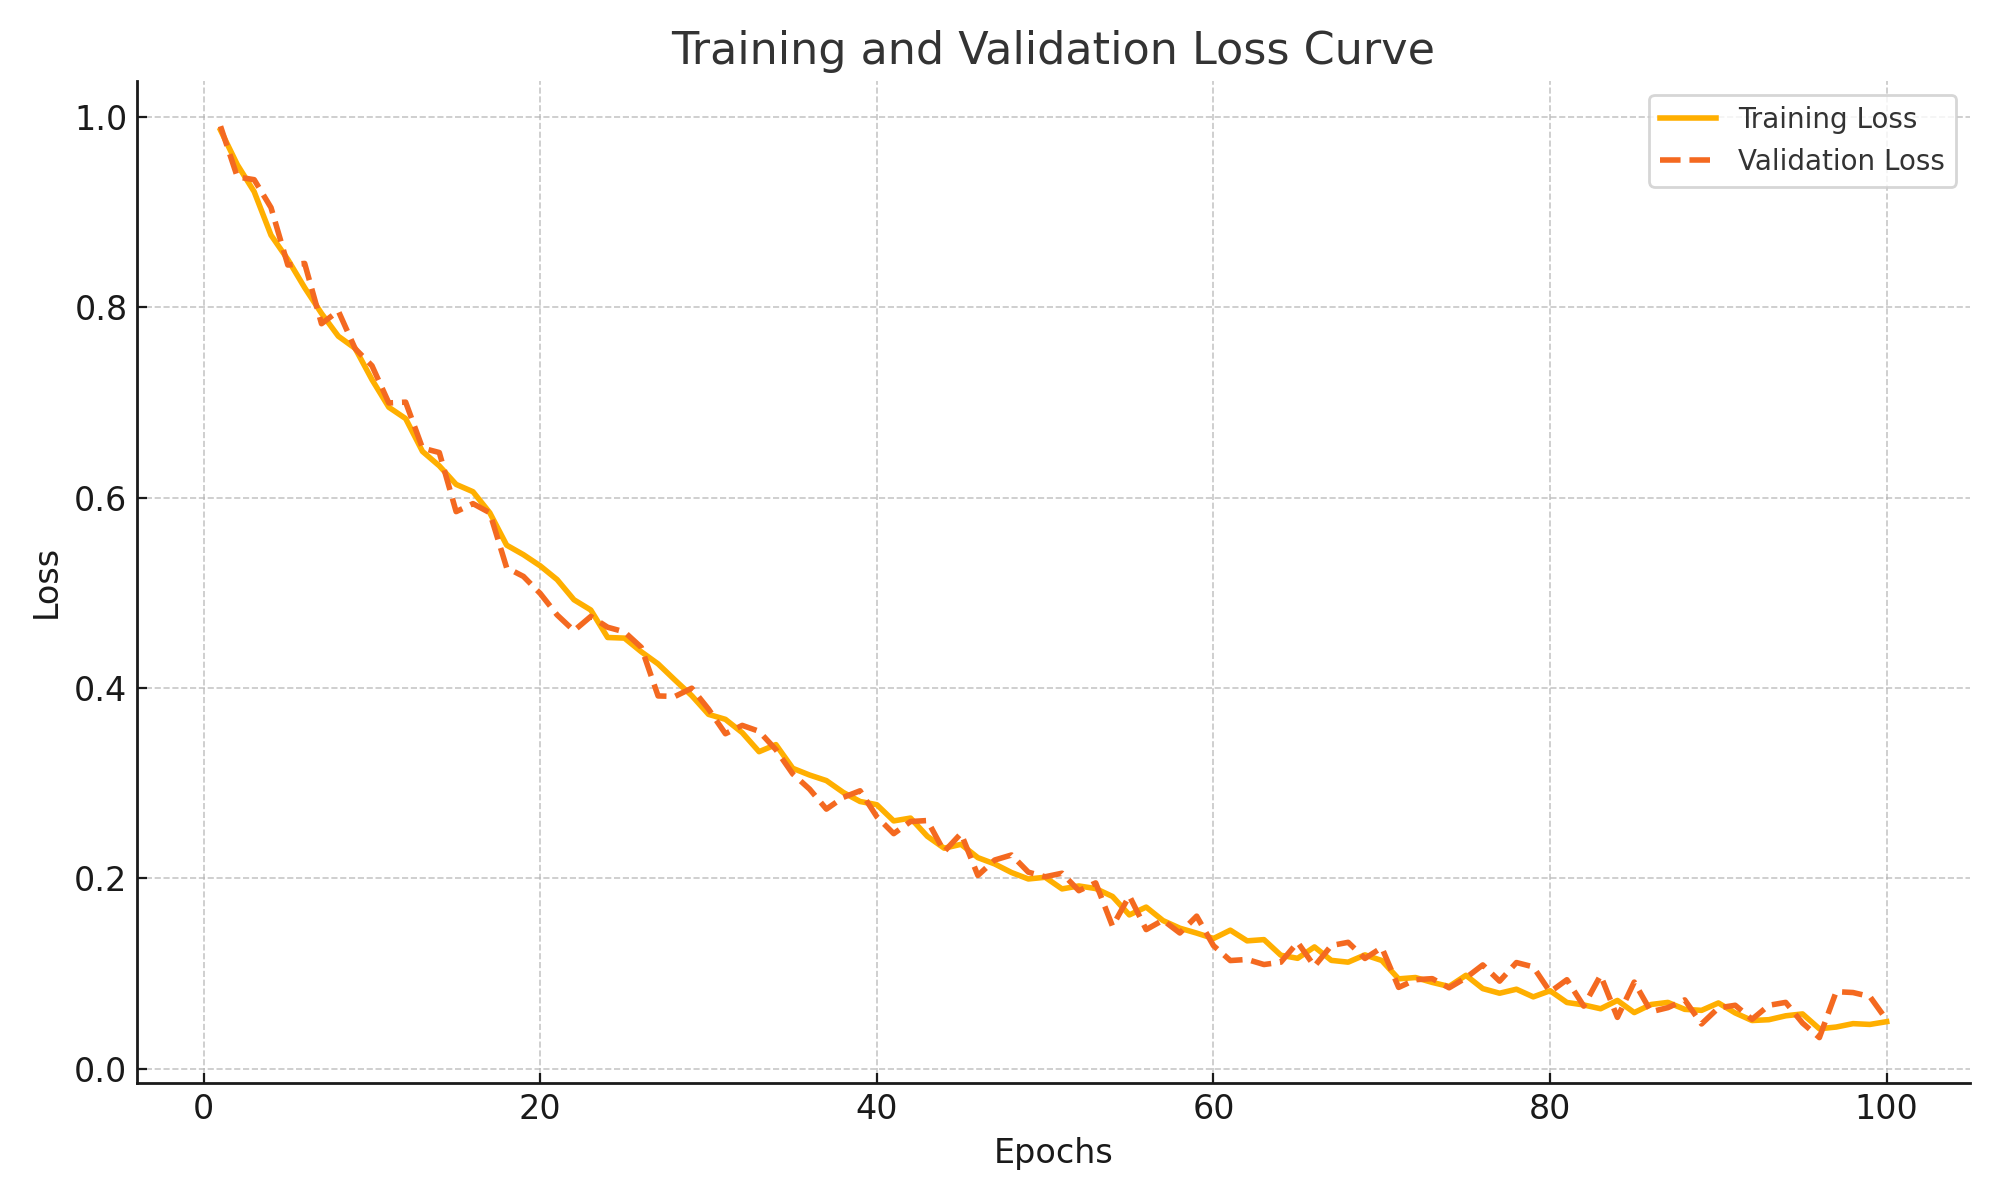
\includegraphics[width=0.8\textwidth]{figures/loss_curve.png}
\caption{Training and Validation Loss Curve}
\label{fig:loss_curve}
\end{figure}

As shown in Figure~\ref{fig:loss_curve}, both training and validation losses exhibited a decreasing trend over epochs, indicating that the model was learning effectively from the data. There was no significant divergence between training and validation curves, suggesting that overfitting was minimized during training.

The model's performance was evaluated using the Root Mean Squared Error (RMSE) metric, which measures the average magnitude of errors between actual and predicted house prices. The results achieved on two major datasets are summarized below:

\begin{table}[h]
\centering
\begin{tabular}{|c|c|}
\hline
\textbf{Dataset} & \textbf{RMSE Value} \\
\hline
New York City (NYC) & 21.43 \\
\hline
Beijing & 60.19 \\
\hline
\end{tabular}
\caption{Model Evaluation Results (RMSE)}
\label{tab:rmse_results}
\end{table}

The RMSE value of 21.43 on the NYC dataset and 60.19 on the Beijing dataset demonstrates that the model achieved reasonable predictive accuracy. Lower RMSE values indicate better performance, meaning the predicted house prices were close to the actual values.

To further analyze the model's effectiveness, a scatter plot was generated comparing actual house prices to predicted prices. Ideally, the points should align closely along the diagonal line, indicating accurate predictions.

\begin{figure}[h]
\centering
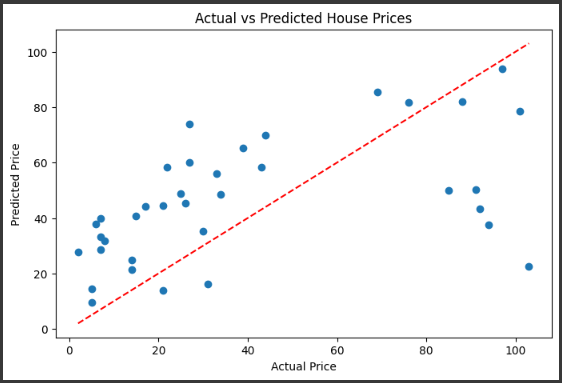
\includegraphics[width=0.8\textwidth]{figures/Screenshot_41.png}
\caption{Actual vs Predicted House Prices}
\label{fig:scatter_plot}
\end{figure}

As observed in Figure~\ref{fig:scatter_plot}, most points are closely aligned along the reference line, although some deviations are present. This behavior suggests that while the model performs well overall, there are a few instances where the predicted prices deviate from the actual values, particularly in extreme price ranges.

Overall, the experimental results validate the proposed approach, and provide a solid baseline for future improvements, such as incorporating multi-modal feature extraction and attention-based fusion mechanisms to further enhance accuracy.
